\section{Methodology validation}
In this chapter, the proposed methodology will be validated, developing a map three-dimensional and a digital elevation model with the Agisoft Photoscan.
\subsection{Surveying area and user input}
\subsubsection{Study area}

All the flight test were carried out in the Odense model airfield, situated 20km north of city. The field has an approximated are of around 74400 $m^2$. figure \ref{fig:Airfield} shows a satellite image of the airfield
\begin{figure}[H]
\centering
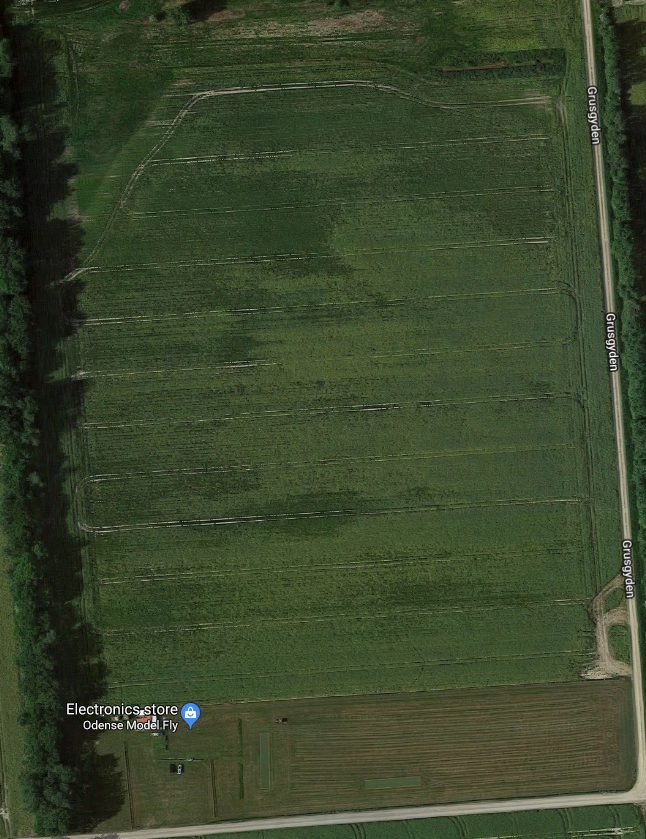
\includegraphics[width=6cm,height=6cm,keepaspectratio]{imagenes/Satellite.png}
\caption{Satellite view of Odense model airfield}
\label{fig:Airfield}
\end{figure}

There are two different study area in the field one two the left (Field A), the other to the right (Field B) of the field. The figure \ref{fig:Study area} shows two study areas delimited by a blue line,the table \ref{table: Area_char} presents details of the study areas.
\begin{figure}[H]
\centering
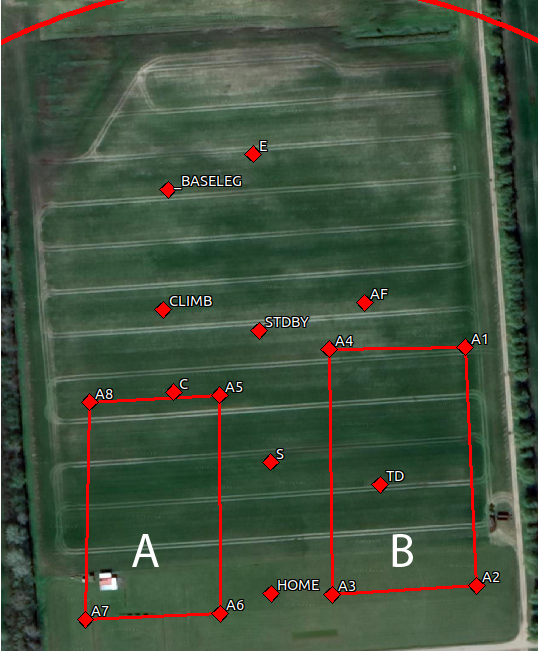
\includegraphics[width=6cm,height=6cm,keepaspectratio]{imagenes/Study_Area.png}
\caption{Study area for the project}
\label{fig:Study area}
\end{figure}

\begin{table}[H]
\centering
\begin{tabular}{|c|c|c|c|c|}
\hline
Area & Length X (m) & Length Y (m) & Area ($m^2$) & Elevation (MAMSL) \\ \hline
A     & 74           & 113         &  8362     & 0                 \\ \hline
B     & 75           & 105          & 7875      & 0                 \\ \hline
\end{tabular}
\caption{Study area characteristics}
\label{table: Area_char}
\end{table}
\subsubsection{Hardware description}
\textit{Ground segment:}
In this section can be found a description of the hardware used to preform the studies.
The ground segment hardware is described in table \ref{Table:Ground_Hardware}
\begin{table}[H]
\centering
\begin{tabular}{|c|c|}
\hline
Hardware             & Description                            \\ \hline
Ground Computer      & Macbook Pro running Ubuntu 18.04.1 LTS \\ \hline
Ground software      & Paparazzi UAS                          \\ \hline
Ground side data link & Xbee Pro 2.4GHz, 18 dBm (63mW)         \\ \hline
Ground side safe link  & Futaba T-FHSS 14 Channels               \\ \hline
\end{tabular}
\caption{Ground segment hardware}
\label{Table:Ground_Hardware}
\end{table}


\textit{Data link:}
Both up and down link use \textit{XBee Pro S1}. the performance specification can be found in table \ref{Table:XBee}
\begin{table}[H]
\centering
\begin{tabular}{|c|c|}
\hline
Specification           & Description   \\ \hline
Range                    & 1600 m        \\ \hline
transmit power output    & 63mW (18 dBm) \\ \hline
RF data rate             & 250000 b/s    \\ \hline
Receiver sensitivity     & 100 dBm       \\ \hline
Operating frequency band & 2.4GHz ISM    \\ \hline
\end{tabular}
\caption{Data link segment hardware specification}
\label{Table:XBee}
\end{table}

\textit{Air segment:} Table \ref{Table:Air_Segment} details the air segment specification 
\begin{table}[H]
\centering
\begin{tabular}{|c|c|}
\hline
Hardware                             & Description                                                                                                                                                          \\ \hline
Airplane                             & Opterra 2m                                                                                                                                                           \\ \hline
Autopilot                            & \multirow{3}{*}{ENAC Apogee autopilot with Paparazzi UAV}                                                                                                          \\ \cline{1-1}
IMU                                  &                                                                                                                                                                      \\ \cline{1-1}
\multicolumn{1}{|l|}{Altitud sensor} &                                                                                                                                                                      \\ \hline
GPS Receiver                         & NEO-M8T GPS + Magnetometer (Error: X,Y +- 4m, Z 4m)                                                                                                                                          \\ \hline
Data link modem                      & XBee Pro S1                                                                                                                                                          \\ \hline
RC reveicer                          & Futaba FASST                                                                                                                                                         \\ \hline
Servos                               & 2x 90 degree servos                                                                                                                                                  \\ \hline
Propultion type                      & 1300 Kv brushless motor with a 40A ESC                                                                                                                               \\ \hline
Batteries                            & 3 cell 3300mAh LiPo                                                                                                                                                  \\ \hline
Paylod                               & \begin{tabular}[c]{@{}c@{}}JeVois smart camera:\\ Focal length: 4.85mm\\ Resolution: 1280x1024\\ Sensor area: 4.13mmx3.28mm\\ Pixel size: 3.25$\mu$mx3.25$\mu$m\end{tabular} \\ \hline
\end{tabular}
\caption{Air segment hardware description}
\label{Table:Air_Segment}
\end{table}

\subsection{Missions}
This section explains the mission procedure and simulation.
\subsubsection{Flight planning variable computation}
The mission consists of surveying study area B with a 0-degree angle (South to North), and area A with a 180-degree angle (North-South). Using the equation from the Flight planning chapter with the parameters of tables. It is possible to compute the following (Front overlap and side overlap for both missions are 80\% , and GSD of 3.5 cm/pixel). Table \ref{Table: Valores} show the computed values:

\begin{table}[H]
\centering
\begin{tabular}{|c|c|c|}
\hline
Parameter                 & Field A & Field B \\ \hline
Space Between lines       & 9 m     & 9 m     \\ \hline
Distance between photos  & 7.2 m   & 7.2m    \\ \hline
Number of photos per line & 19      & 16      \\ \hline
Number of lines           & 9       & 8       \\ \hline
Flight altitude            & 50      & 50      \\ \hline
\end{tabular}
\caption{Value computation for flight planning}
\label{Table: Valores}
\end{table}

\subsubsection{Mission simulation}
The simulation of the mission is executed on the Paparazzi Ground Control Station (GCS). Compiling the mission code in NPS mode, it is possible to estimate the plane behavior and path. Figure \ref{fig:bsim} shows the simulation of Field B surveying mission.
\begin{figure}[H]
\centering
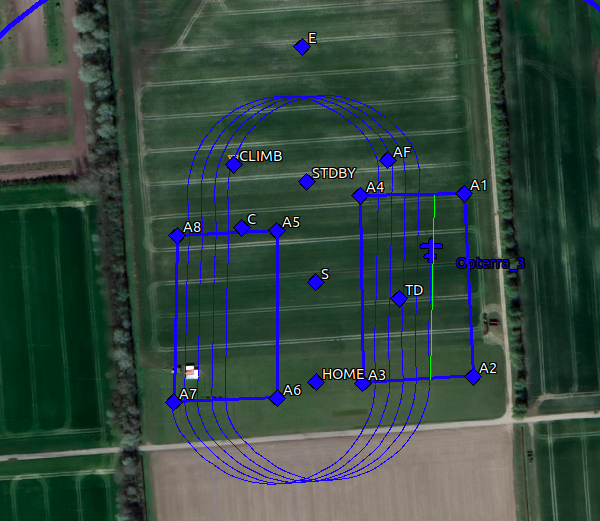
\includegraphics[width=10cm,height=10cm,keepaspectratio]{imagenes/SimBField.png}
\caption{B field surveying mission simulation}
\label{fig:bsim}
\end{figure}
The result of the simulation are displayed in table \ref{Table:SimResult}
\begin{table}[H]
\centering
\begin{tabular}{|c|c|c|c|}
\hline
Surveying Field & Number of photos & Number of strips & Execution time \\ \hline
A               & 125              & 8                & 7:10           \\ \hline
B               & 146              & 9                & 7:30           \\ \hline
\end{tabular}
\caption{Result of surveying mission simulation}
\label{Table:SimResult}
\end{table}
